\documentclass{article}
\usepackage{tikz}
\usetikzlibrary{automata, positioning, arrows}

\usepackage[letterpaper, margin=1.5in]{geometry}
\usepackage{setspace}
\doublespacing
\usepackage[utf8]{inputenc}
\usepackage[
backend=biber,
style=alphabetic,
sorting=ynt
]{biblatex}
\usepackage{tipa}
\usepackage{gb4e}
\addbibresource{refs.bib}

\title{Final Obstruent Gemination in Japanese Loanwords}
\author{Derek Andersen}
\date{March 12, 2020}

\begin{document}
\tikzset{
->, % makes the edges directed
node distance=3cm, % specifies the minimum distance between two nodes. Change if necessary.
every state/.style={thick, fill=gray!10}, % sets the properties for each ’state’ node
initial text=$ $, % sets the text that appears on the start arrow
}
\maketitle

\section{Introduction}
Japanese loanwords provide a rich source of data for the analysis of the gemination of certain consonantal segments in Japanese, and in  particular, the types of segments for which Japanese phonology allows gemination. In this paper I will provide a computational analysis of the process of gemination in some Japanese loanwords, drawing on formulas of First Order logic. My analysis will focus particularly on the process of word-final obstruent gemination, e.g. /p/, /t/, /k/, /b/, /d/, and /g/. As we will see, in addition to the type of segment in question, the length of the preceding vowel also plays a role in whether gemination is licensed. In section \ref{gemprocess}, I introduce the process of word-final obstruent gemination and provide some examples, and in section \ref{logical}, I present a logical analysis for the gemination transformation using First Order logic with the successor relation.

\section{The gemination process}
\label{gemprocess}
The native phonemic inventory of Japanese consists of singleton consonants (like /p/, /t/, /k/) as well as geminate consonants (like /pp/, /tt/, /kk/). As shown by the minimal pair data in \ref{minimalpair}, they are contrastive, and thus separate phonemes. \cite{Kubozono2009}

\begin{exe}
    \ex
    \label{minimalpair}
    \begin{itemize}
        \item [a] /kita/ ‘came' vs. /kitta/ ‘cut (past)'
        \item [b] /saki/ ‘point' vs. /sakki/ ‘a short time ago'
    \end{itemize}
    
\end{exe}

Gemination in Japanese loanwords behaves similarly to its native counterpart process, with an extension to allow for voiced obstruent gemination (which is not attested natively). Specifically, words like ‘red' (assuming an input form of /red/ in Japanese) when borrowed into Japanese will have their final consonant geminated (in this case, to [reddo]) in the output. For the purposes of my analysis, I will disregard the final vowel epenthesis in all cases of loanword phonemicization, as it does not speak to the gemination process. Examples of word-final obstruent gemination cases are shown in \ref{short}. \cite{Kawahara2015}

\begin{exe}
    \ex
    \label{short}
    \begin{itemize}
        \item [a] ‘ca\textbf{t}' $\rightarrow$ [ka\textbf{tt}o]
        \item [b] ‘pa\textbf{ck}' $\rightarrow$ [pa\textbf{kk}u]
        \item [c] ‘bi\textbf{g}' $\rightarrow$ [bi\textbf{gg}u]
    \end{itemize}
\end{exe}

There is also a stipulation which states that for word-final obstruent gemination to occur, the preceding vowel must be short in length. In other words, word-final obstruent gemination is not licensed when the preceding vowel is long, as in the examples in \ref{long}. \cite{Kubozono2009}

\begin{exe}
    \ex
    \label{long}
    \begin{itemize}
        \item [a] ‘mea\textbf{t}' $\rightarrow$ [mii\textbf{t}o] \hspace{1cm} *[mii\textbf{tt}o]
        \item [b] ‘pea\textbf{k}' $\rightarrow$ [pii\textbf{k}u] \hspace{1cm} *[pii\textbf{kk}u]
        \item [c] ‘par\textbf{k}' $\rightarrow$ [paa\textbf{k}u] \hspace{1cm} *[paa\textbf{kk}u]
    \end{itemize}
\end{exe}

\section{Logical analysis}
\label{logical}
\subsection{Defining a model for ‘pack'}
For the purposes of this logical analysis of the transformations at work, I will assume the input to be the surface phonetic form of the word in the original language (in this case, English). Importantly, I will be ignoring the vowel change between [æ] $\rightarrow$ [a] in ‘pack', shown below in \ref{vowel}. This phonemicized form will be used as our input for the word-final obstruent gemination transformation. Again, the final vowel epenthesis is not being considered for this analysis and should be disregarded.
\pagebreak

\begin{exe}
    \ex
    \label{vowel}
    \begin{itemize}
        \item [] \hspace{33} \textbf{Source} \hspace{25} \textbf{Phonemicized} \hspace{29} \textbf{Output}
        \item [] ‘pack' \hspace{4} /pæk/ \hspace{15}  $\rightarrow$ \hspace{15}   /pak/ \hspace{20} $\rightarrow$ \hspace{20} [pakk(u)]
    \end{itemize}
\end{exe}

Thus, considering the word ‘pack', the input for the transformation for this word will be /pak/. Our goal will be to define a logical model for a transformation that will account for the output [pakk] from the input /pak/. For this purpose I will be utilizing a model of First Order logic with the successor relation, and its signature is in \ref{model}. Included in this signature are the unary relations \textit{p}, \textit{a}, and \textit{k} because they are necessary to express the transformation from input to output, as we will see. Omitted for readability are the remaining segments of Japanese, including but not limited to the obstruents that would undergo gemination in the same context (/t/, /b/, /d/, /g/) as well as other vowels.

\begin{exe}
    \ex
    \label{model}
    \begin{itemize}
        \item [] $M^\triangleleft := \langle D; \triangleleft, p, a, k \rangle $
    \end{itemize}
\end{exe}

The transformation that I will be using to account for the gemination process is a copying transformation which relies on the use of a copyset, $C$. Through the use of a copyset, the input (copy 1) can be “copied" into the output (copy 2), and the formulas I define will license the transformation in question. In section \ref{copysection}, the use of copies will make clear the intuition behind the choice of using the successor relation in our model.

The first formulas that I will define as part of my logical model will be the unary relations for \textit{p}, \textit{a}, and \textit{k}. These are listed in \ref{unary}. To denote the formulas which refer to the relations in copy 2 vs. copy 1, I use a superscript $^2$. These copies will be discussed further in section \ref{copysection}.

\begin{exe}
    \ex
    \label{unary}
    \begin{itemize}
        \item [a] $\varphi_{p}^1(x) := p(x)$
        \item [b] $\varphi_{p}^2(x) := False$
        \item [c] $\varphi_{a}^1(x) := a(x)$
        \item [d] $\varphi_{a}^2(x) := False$
        \item [e] $\varphi_{k}^1(x) := k(x)$
        \item [f] $\varphi_{k}^2(x) := \texttt{obstruent}(x) \wedge \texttt{last}(x) \wedge \texttt{after\_short}(x)$
    \end{itemize}
\end{exe}

Using \ref{unary}a as an example, these formulas state something along the lines of the following: “If $x$ is a \textit{p} in the input, it will be a \textit{p} in the output (in this case, of copy 1)." This necessarily means that in the cases of \ref{unary}b and \ref{unary}d, the formulas state that input \textit{p}s and \textit{a}s will not carry over to the output (of copy 2). Furthermore, according to \ref{unary}f, it is the case that input \textit{k}s will appear in the output (of copy 2) iff the user-defined predicates \texttt{obstruent}, \texttt{last}, and \texttt{after\_short} defined in \ref{obs}, \ref{last}, and \ref{aftershort} are satisfied by $x$.

\begin{exe}
    \ex
    \label{obs}
    \begin{itemize}
        \item [] $\texttt{obstruent}(x) := p(x) \vee t(x) \vee k(x) \vee b(x) \vee d(x) \vee g(x)$
    \end{itemize}
\end{exe}

\begin{exe}
    \ex
    \label{last}
    \begin{itemize}
        \item [] $\texttt{last}(x) := \neg \exists y (x \triangleleft y)$
    \end{itemize}
\end{exe}

\begin{exe}
    \ex
    \label{aftershort}
    \begin{itemize}
        \item [] $\texttt{after\_short}(x) := \exists y (\texttt{short\_vowel}(y) \wedge y \triangleleft x)$
    \end{itemize}
\end{exe}

\begin{exe}
    \ex
    \label{shortvowel}
    \begin{itemize}
        \item [] $\texttt{short\_vowel}(x) := a(x) \vee i(x) \vee u(x) \vee e(x) \vee o(x)$
    \end{itemize}
\end{exe}

Predicate \ref{obs} states that if $x$ is any of the symbols \textit{p}, \textit{t}, \textit{k}, \textit{b}, \textit{d}, \textit{g}, then $x$ is an obstruent, while predicate \ref{last} states that if there is no such $y$ such that $y$ is the successor of $x$, then $x$ is the last symbol in the string. Predicate \ref{aftershort} draws upon predicate \ref{shortvowel} to state that if there exists a $y$ such that $y$ is a short vowel and $x$ succeeds $y$, then $x$ has the property of being after a short vowel, importantly giving us the power to express which symbols will be licensed for gemination. Note here that “short" refers to vowels which are not “long", denoted by a double /aa/ vs. a single /a/, for example.

\subsection{The copyset and binary relations}
\label{copysection}
The mechanism which will make my analysis of the gemination process possible is the copyset, $C$, defined in \ref{copyset}.

\begin{exe}
    \ex
    \label{copyset}
    \begin{itemize}
        \item [] $C := \{1, 2\}$
    \end{itemize}
\end{exe}

Each element in the copyset will generate an output copy of our input string, ‘pak', which is illustrated in Figure 1.

\pagebreak

\begin{figure}
    \centering
    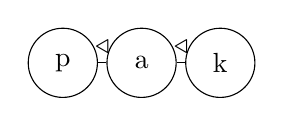
\begin{tikzpicture}
        \node[state] (q1) {p};
        \node[state, right of=q1] (q2) {a};
        \node[state, right of=q2] (q3) {k};
       
        \draw   (q1) edge [above] node{$\triangleleft$} (q2)
                (q2) edge [above] node{$\triangleleft$} (q3);
                
    \end{tikzpicture}
    \caption{Input representation of ‘pak' under our successor model}
\end{figure}

Before copies 1 and 2 can be introduced, I must define the formulas for the binary successor relation in our model for ‘pak'. These are in \ref{binary}, and they are denoted by superscript pairs of 1 and 2, which indicate the directionality of the successor relation for the arguments in the formula.

\begin{exe}
    \ex
    \label{binary}
    \begin{itemize}
        \item [a] $\varphi_{\triangleleft}^{1,1}(x, y) := x \triangleleft y$
        \item [b] $\varphi_{\triangleleft}^{1,2}(x, y) := \texttt{last}(x) \wedge \texttt{last}(y) \wedge x \triangleleft y$
        \item [c] $\varphi_{\triangleleft}^{2,1}(x, y) := False$
        \item [d] $\varphi_{\triangleleft}^{2,2}(x, y) := x \triangleleft y$ 
    \end{itemize}
\end{exe}

Now we can look at the representation of the output strings for copies 1 and 2, and drawing upon the formulas defined in \ref{unary} (the unary relations) and \ref{binary} (the binary relations), we can explain the transformation taking place which results in /pak/ $\rightarrow$ [pakk]. Crucially, what our binary relation formulas do is provide criteria for which successor relations will hold in the final output, which can be thought of as a “combination" of copy 1 and copy 2. The formulas in \ref{binary} are clarified below.

\begin{itemize}
    \item [\textbf{\ref{binary}a}] Across members of copy 1, members which are in the successor relation will remain so
    \item [\textbf{\ref{binary}b}] Between members of copy 1 $\rightarrow$ copy 2, if $x$ is the last element of a copy and $y$ is the last element of a copy, then $x$ is succeeded by $y$
    \item [\textbf{\ref{binary}c}] Between members of copy 2 $\rightarrow$ copy 1, no successor relations hold
    \item [\textbf{\ref{binary}d}] Across members of copy 2, members which are in the successor relation will remain so
\end{itemize}

What this entails is that in copy 2 (shown in Figure 3), $\o$  is succeeded by $\o$ which is succeeded by \textit{k}, which is necessarily true if ‘\o' is treated as \textit{nothing}. It is precisely for this reason that \ref{binary}b holds, which allows the successor relation from copy 1 $\rightarrow$ copy 2 to “skip" positions 1 and 2 in copy 2, and consider only position 3 which is occupied by the \textit{k}.

\pagebreak
\begin{figure}[ht]
    \centering
    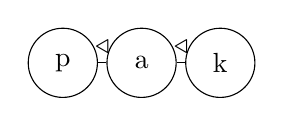
\begin{tikzpicture}
        \node[state] (q1) {p};
        \node[state, right of=q1] (q2) {a};
        \node[state, right of=q2] (q3) {k};
       
        \draw   (q1) edge [above] node{$\triangleleft$} (q2)
                (q2) edge [above] node{$\triangleleft$} (q3);
                
    \end{tikzpicture}
    \caption{Output representation of copy 1 of ‘pak'}
\end{figure}

\begin{figure}[ht]
    \centering
    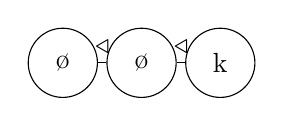
\begin{tikzpicture}
        \node[state] (q1) {\o};
        \node[state, right of=q1] (q2) {\o};
        \node[state, right of=q2] (q3) {k};
       
        \draw   (q1) edge [above] node{$\triangleleft$} (q2)
                (q2) edge [above] node{$\triangleleft$} (q3);
                
    \end{tikzpicture}
    \caption{Output representation of copy 2 of ‘pak'}
\end{figure}

The final two formulas that are needed are ones that will allow, or license, the segments which are acceptable in the output [pakk]. Since we have two copies, we will need to define two separate licensing formulas, one for each copy. These are defined in \ref{license}.

\begin{exe}
    \ex
    \label{license}
    \begin{itemize}
        \item [a] $\varphi_{license}^{1}(x) := True$
        \item [b] $\varphi_{license}^{2}(x) := \texttt{obstruent}(x) \wedge \texttt{last}(x)$
    \end{itemize}
\end{exe}

The formula in \ref{license}a simply states that segments in copy 1 are always licensed. In \ref{license}b, however, the formula restricts licensed segments to those which satisfy \texttt{obstruent} and \texttt{last}. In the case of [pakk], the first [p], [a], and [k] are elements of the first copy, and thus are all licensed, and the second [k] is (1) a member of the second copy, (2) an obstruent, and (3) the last segment of its copy. For these reasons, the final [k] is licensed. Crucially, what allows for the correct order of the output segments is the binary successor relations defined in \ref{binary}. The final output representation of [pakk] is illustrated in Figure 4.

\begin{figure}[ht]
    \centering
    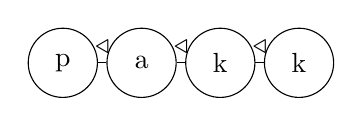
\begin{tikzpicture}
        \node[state] (q1) {p};
        \node[state, right of=q1] (q2) {a};
        \node[state, right of=q2] (q3) {k};
        \node[state, right of=q3] (q4) {k};
       
        \draw   (q1) edge [above] node{$\triangleleft$} (q2)
                (q2) edge [above] node{$\triangleleft$} (q3)
                (q3) edge [above] node{$\triangleleft$} (q4);
                
    \end{tikzpicture}
    \caption{Final output representation of [pakk]}
\end{figure}

\section{Conclusion}
We have seen that in certain contexts, Japanese loanwords undergo word-final obstruent gemination. Specifically, when the preceding vowel is short, and the obstruent in question is in the final position in the input string, gemination is licensed. I have presented in this paper a logical analysis of a transformation accounting for this gemination process, drawing upon formulas of First Order logic with the successor relation. It is apparent that in order for our model to successfully account for the process, the successor relation is necessary — it is what allows us to define binary relations between elements of the first copy to the second copy, and account for gemination in the surface form.

\printbibliography
\end{document}